\documentclass[11pt]{article}
\title{\textbf{CS 361 Spring 2018\\Homework 10}}
\author{Nathaniel Murphy (njmurph3)}
\date{}

\usepackage{a4wide}
\usepackage{amsfonts}
\usepackage{amsmath}
\usepackage{amsthm}
\usepackage{graphicx}

\begin{document}
\maketitle
\section*{11.1}
For this classifier, I first created a list of normal models for each feature using the library \texttt{norm} from the \texttt{scipy.stats} package. The \texttt{get\_models} function is essentially the training function for the classifier. All we need to do to predict future values is obtain the normal models for each feature. Once we want to predict future values, for each new example, we can predict the probability that that example falls within a certain class by obtaining probabilities that every feature in that example follows the normal models for that class. I was able to obtain a 74.67\% accuracy for the test dataset.
\section*{11.4}
\subsection*{(a)}
\begin{figure}[h!]
	\centering
	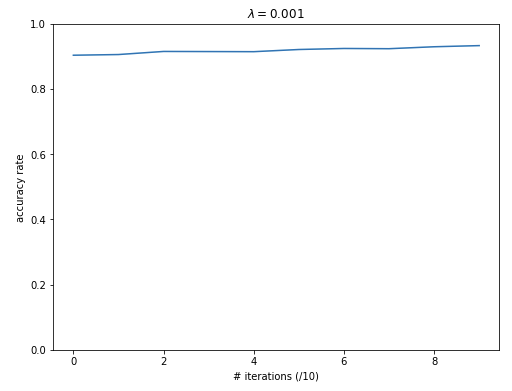
\includegraphics[width=125mm]{graph_1.png}
\end{figure}
\clearpage
\begin{figure}[h!]
	\centering
	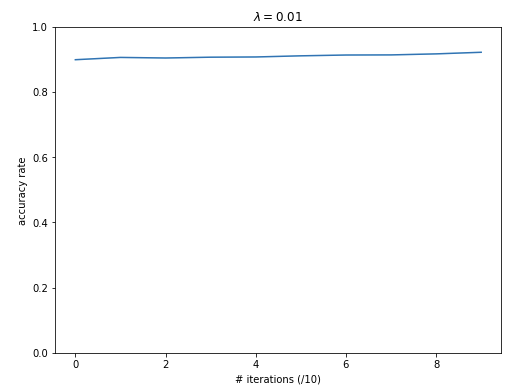
\includegraphics[width=125mm]{graph_2.png}
\end{figure}
\begin{figure}[h!]
	\centering
	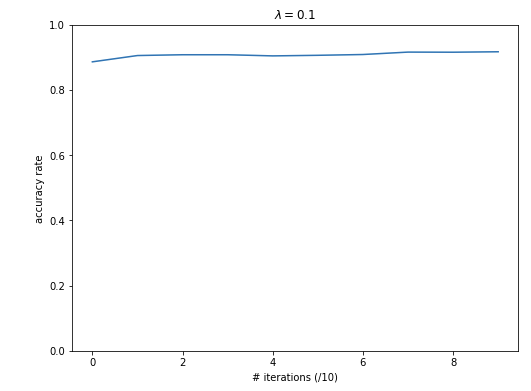
\includegraphics[width=125mm]{graph_3.png}
\end{figure}
\clearpage
\begin{figure}[h!]
	\centering
	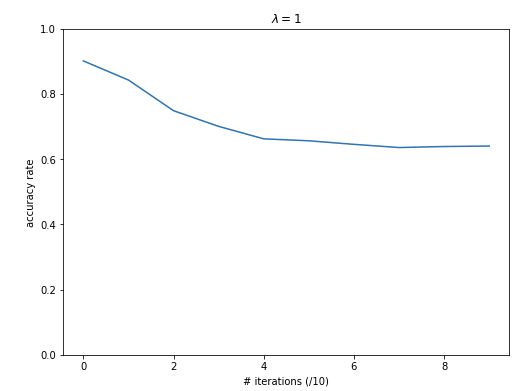
\includegraphics[width=125mm]{graph_4.png}
\end{figure}
\ \\
\subsection*{(b,c)}
What I did was kept track of all of the accuracies for every epoch for each of the regularization constants. After running all epochs, for each regularization constant, I averaged the accuracies for every 10 iterations and plotted them above. \\ \\
It looks as if using the $\lambda=0.001$ regularization constant will give us the best results with our model because, compared with the $\lambda=0.1$ and $\lambda=1$ models, the $\lambda=0.001$ does have significant improvement (the $\lambda=1$ accuracy even decreases!). The $\lambda=0.01$ and $\lambda=0.001$ models are very close, but the $\lambda=0.001$ model ended up having a slightly higher accuracy. Using the $\lambda=0.001$ model, we estimated an accuracy metric for this classifier. We see that we can achieve around a 92\% accurate classifier using an SVM for this problem.
\section*{11.7}
\begin{figure}[h!]
	\centering
	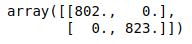
\includegraphics[width=50mm]{ccm.png}
	\caption{Class Confusion Matrix for the mushroom data}
\end{figure}
\ \\
Taking the vertical axis to represent the truth of the values and the horizontal axis to represent predicted values, we see that we have classified all of the values correctly, and thus, there is no way that a mushroom that we predicted edible will actually be poisonous.
\end{document}